\chapter{Auswertung der Performancetests}
\label{AuswertungderPerformancetests}
In diesem Kapitel werden die Performancetests, die mit Apache JMeter mit den jeweiligen Testplänen durchgeführt wurden, ausgewertet. Es wurden drei Testpläne durchgeführt, Lasttest, Skalierbarkeitstest sowie der Stresstest und zu jedem Test folgt eine Auswertung. Diese Auswertung wird vergleichend betrachtet, da es zwei Ressource Server gibt, auf denen die Tests jeweils angewandt wurden, nämlich einmal der Ressource Server, der die Zugriffskontrolle mit Open Policy Agent entkoppelt und der zweite Ressource Server, der die Zugriffskontrolle in dem Server selbst implementiert. Der HTML-Report, der von Apache JMeter aus den Messwerten in der csv-Datei erstellt wird, gibt eine Reihe von Grafiken und Statistiken aus anhand dessen die Auswertung geschieht.\smallskip

Es ist wichtig zu erwähnen, dass die Messergebnisse in einem Testumfeld zustande gekommen sind, in dem sich Client und Server in demselben Netzwerk befinden. Dadurch entsteht zwischen beiden Systemen durch die Entfernung beider Systeme zueinander keine nennenswerte Latenz. Typischerweise befinden sich im Praxiseinsatz Client und Server nicht in demselben Netzwerk, sondern sie befinden sich in unterschiedlichen Netzwerken und sind geographisch über eine gewisse Entfernung voneinander entfernt. Dadurch entsteht eine entfernungsabhängige Latenz bei der Kommunikation zwischen Systemen, diese ist hier bei den Messergebnissen nicht mitinbegriffen. Das Anpingen von handelsüblichen deutschen Webseiten, ergibt eine Latenz von ca. 20 Millisekunden, wobei auch dies stark von der Internetverbindung abhängt. Eine spezifische Latenz kann auf die Messergebnisse in den nachfolgenden Kapiteln hinzugerechnet werden.

\section{Lasttest}
In diesem Test wurden zehn Threads, die jeweils kontinuierlich HTTP Anfragen mit validen JSON Web Token an den Server senden, über einen Zeitraum von 15 Minuten gestartet. Es stellte es sich heraus, dass der Server, der die Zugriffskontrolle mit Open Policy Agent entkoppelt, eine durchschnittlich 3,36-mal höhere Response Time aufweist im Vergleich zu dem Server, der die Zugriffskontrolle nicht entkoppelt.\smallskip

Zunächst werden die Messergebnisse von der Spring-Boot Applikation dargestellt, die eine rollenbasierte Zugriffskontrolle mittels dem JwtAuthenticationConverter realisiert hat. Dies ist der Server, der die Zugriffskontrolle in dem Server selbst implementiert. 

\begin{figure}[H]
  \centering
  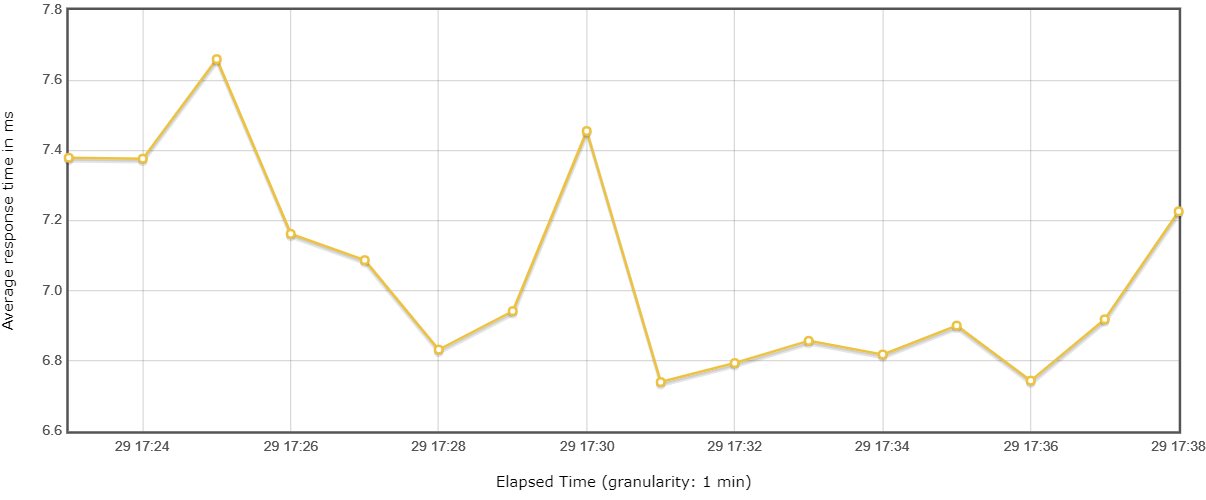
\includegraphics[width=1.0\textwidth]{gfx/flotResponseTimesOverTime.png}
  \caption{Response Time Graph von Lasttest von Ressource Server ohne OPA}
  \label{fig:chapter04:flotResponseTimesOverTime}
\end{figure}

In \autoref{fig:chapter04:flotResponseTimesOverTime} ist ein Diagramm dargestellt, das die durchschnittliche Response Time von dem Ressource Server ohne Open Policy Agent über den gesamten Zeitraum des Lasttests darstellt. Auf der x-Achse ist die Zeit und auf der y-Achse die durchschnittliche Response Time zu dem jeweiligen Zeitpunkt. Es ist zu sehen, dass die Response Time anfangs höher ausfällt und sie kontinuierlich sinkt, bis sie auf ungefähr dem gleichen Niveau verbleibt. Das könnte damit erklärt werden, dass jeder Thread zunächst eine Verbindung durch den 3-Way-Handshake mit dem Server aufbauen muss, welcher zusätzliche Zeit in Anspruch nimmt. Sobald die Verbindung aufgebaut ist, fällt die durchschnittliche Response Time niedriger aus. Über den gesamten Zeitraum bewegen sich aber die Response Times im Bereich zwischen 7,8 Millisekunden und 6,6 Millisekunden. 

\begin{figure}[H]
  \centering
  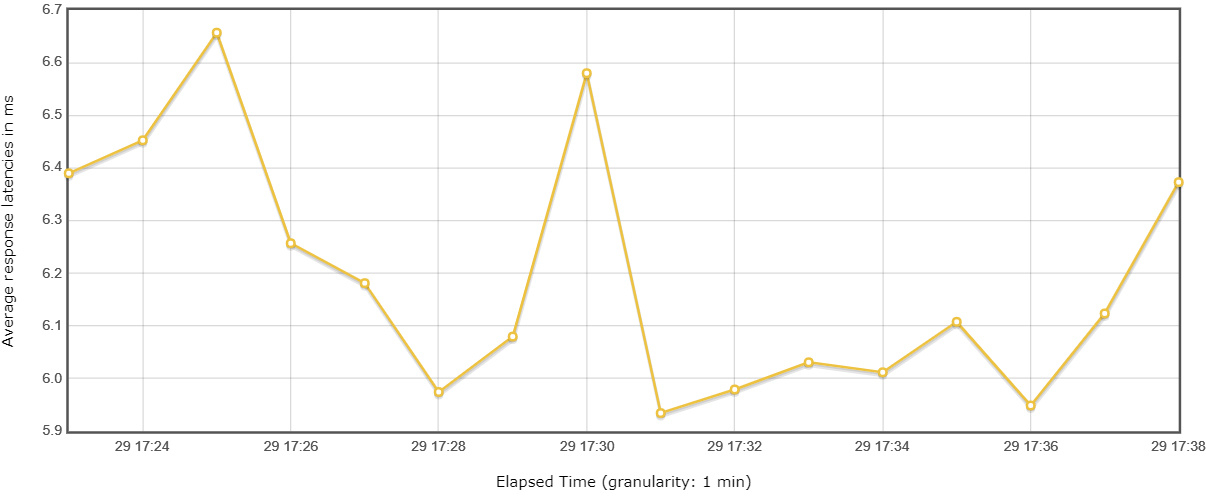
\includegraphics[width=1.0\textwidth]{gfx/flotLatenciesOverTime.png}
  \caption{Latency Time Graph von Lasttest von Ressource Server ohne OPA}
  \label{fig:chapter04:flotLatenciesOverTime}
\end{figure}

In \autoref{fig:chapter04:flotLatenciesOverTime} ist prinzipiell der gleiche Graph dargestellt, nur das hier anstatt der Response Time die Latenz dargestellt ist. Der Unterschied ist hier, wie in \autoref{sec:ApacheJMeterundMetriken} erläutert, dass die Latenz die Zeit von bevor dem Senden der Anfrage bis zum Eintreffen des ersten Bytes der Antwort darstellt, während die Response Time die Zeit bis zum letzten Byte der Antwort misst. Die Latenz ist also immer kürzer als die Response Time. Hier ist zu sehen das zu dem Zeitpunkt 17:38 die Latenz 6,4 Millisekunden beträgt, während zum selben Zeitpunkt die Response Time 7,2 Millisekunden beträgt. In den folgenden Betrachtungen wird allerdings nur noch auf die Response Time eingegangen, da sie die wichtigere Metrik aus Nutzersicht ist, da ein Nutzer eine vollständige Antwort von dem Server haben möchte. Es ist keine zweckmäßige Beurteilung von Antwortzeiten möglich, wenn das erste Byte der Antwort des Servers zeitnah eintrifft, bis zum Eintreffen des letzten Bytes allerdings zwei Stunden vergehen. 

\begin{figure}[H]
  \centering
  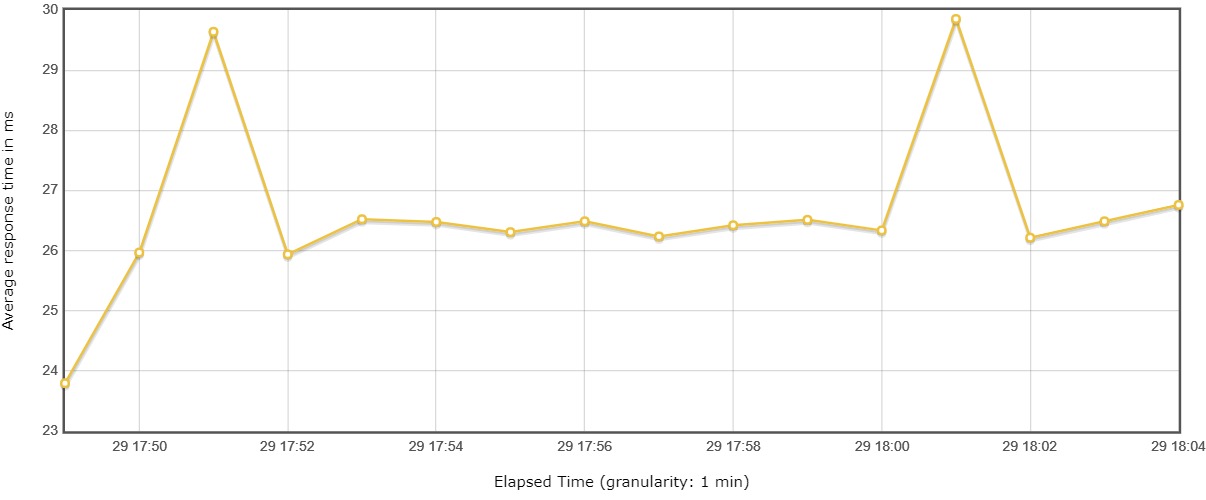
\includegraphics[width=1.0\textwidth]{gfx/flotResponseTimesOverTime-opa-last.png}
  \caption{Response Time Graph von Lasttest von Ressource Server mit OPA}
  \label{fig:chapter04:flotResponseTimesOverTime-opa-last}
\end{figure}

In \autoref{fig:chapter04:flotResponseTimesOverTime-opa-last} ist der Response Time Graph von dem Server dargestellt, der die Zugriffskontrolle mittels Open Policy Agent entkoppelt hat. Auch hier ist die Response Time anfangs höher, bis sie sich auf ein niedrigeres Level einpendelt. Aber das weitaus wichtigere ist, dass die Response Times hier durchschnittlich um ein Vielfaches höher ausfallen als bei dem Server mit interner Zugriffskontrolle. Die meiste Zeit über bewegen sich die Response Times hier zwischen 26 und 30 Millisekunden, während sie bei dem Server mit interner Zugriffskontrolle sich zwischen 6,4 und 7,2 Millisekunden bewegen.\smallskip

Dies ist insofern überraschend, da die Kommunikation, die zwischen Ressource Server und Open Policy Agent auftritt, auf localhost zu localhost Basis verläuft. Das heißt der Ressource Server und Open Policy Agent laufen auf derselben Maschine und es war nicht vorhersehbar, dass durch die HTTP-Kommunikation zwischen diesen beide Komponenten eine derart hohe zusätzliche Latenz entsteht. 

\begin{figure}[H]
  \centering
  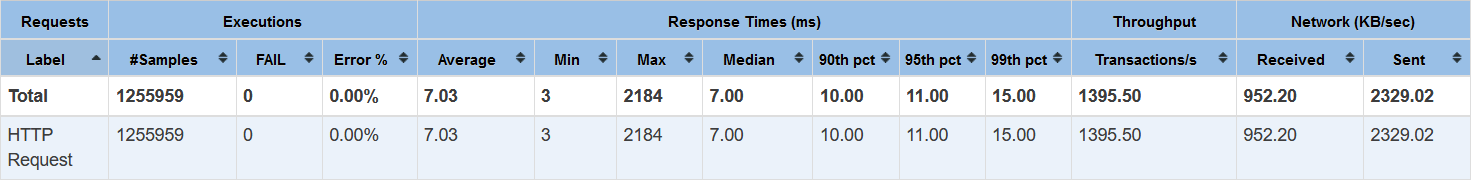
\includegraphics[width=1.0\textwidth]{gfx/statistik-last-noOPA.png}
  \caption{Statistiken von Lasttest von Ressource Server ohne OPA}
  \label{fig:chapter04:statistik-last-noOPA}
\end{figure}

In \autoref{fig:chapter04:statistik-last-noOPA} ist abschließend noch eine statistische Auswertung der Lasttests für den Ressource Server ohne Open Policy Agent zu sehen. Die durchschnittliche Response Time beträgt 7.03 Millisekunden und innerhalb von 15 Minuten wurden 1255959 Anfragen bearbeitet. 

\begin{figure}[H]
  \centering
  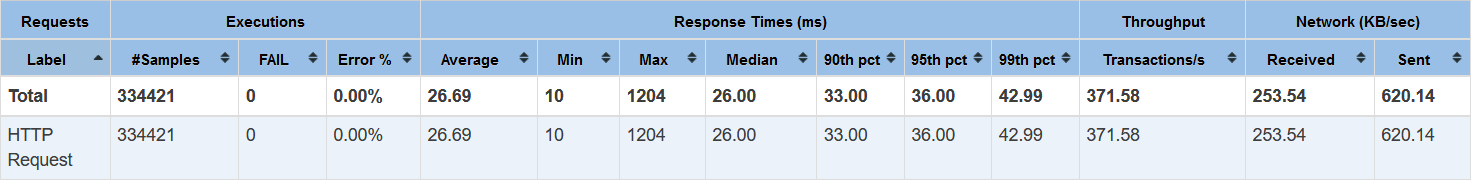
\includegraphics[width=1.0\textwidth]{gfx/statistik-last-opa.png}
  \caption{Statistiken von Lasttest von Ressource Server mit OPA}
  \label{fig:chapter04:statistik-last-opa}
\end{figure}

In \autoref{fig:chapter04:statistik-last-opa} ist die statistische Auswertung der Lasttests für den Ressource Server mit entkoppelter Zugriffskontrolle dargestellt. Hier beträgt die durchschnittliche Response Time 26.69 Millisekunden. Erwähnenswert ist, dass in diesem Test der Server lediglich 334421 Anfragen innerhalb 15 Minuten beantworten konnte. Die durchschnittliche Response Time ist um den Faktor drei höher und entsprechend können auch um etwa um den Faktor drei weniger Anfragen beantwortet werden.

\begin{figure}[H]
  \centering
  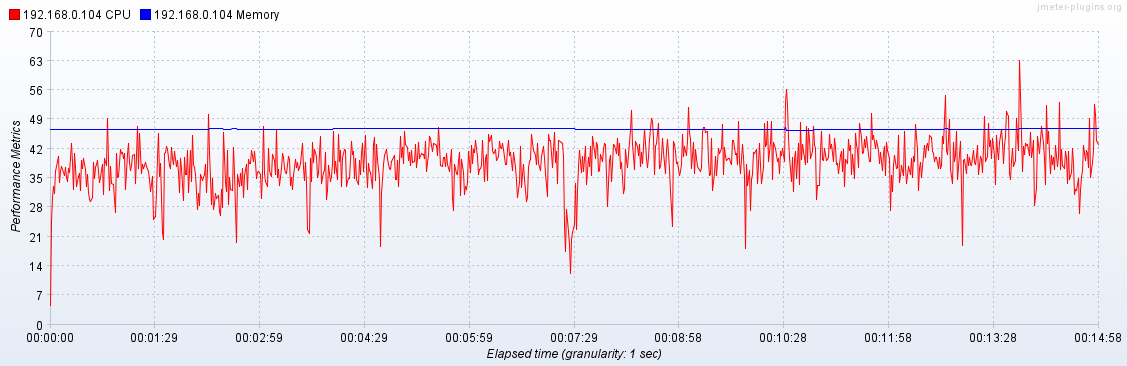
\includegraphics[width=1.0\textwidth]{gfx/perfmon-last-noOPA.png}
  \caption{Perfmon von Lasttest von Ressource Server ohne OPA}
  \label{fig:chapter04:perfmon-last-noOPA}
\end{figure}

In \autoref{fig:chapter04:perfmon-last-noOPA} ist die CPU-Auslastung während des Lasttests für den Ressource Server ohne entkoppelte Zugriffskontrolle zu sehen. Dies ist die rote Linie. Die CPU-Auslastung bewegt sich im Bereich von 42\%. Die RAM-Belegung bleibt konstant, dies ist durch die blaue Linie gekennzeichnet. 

\begin{figure}[H]
  \centering
  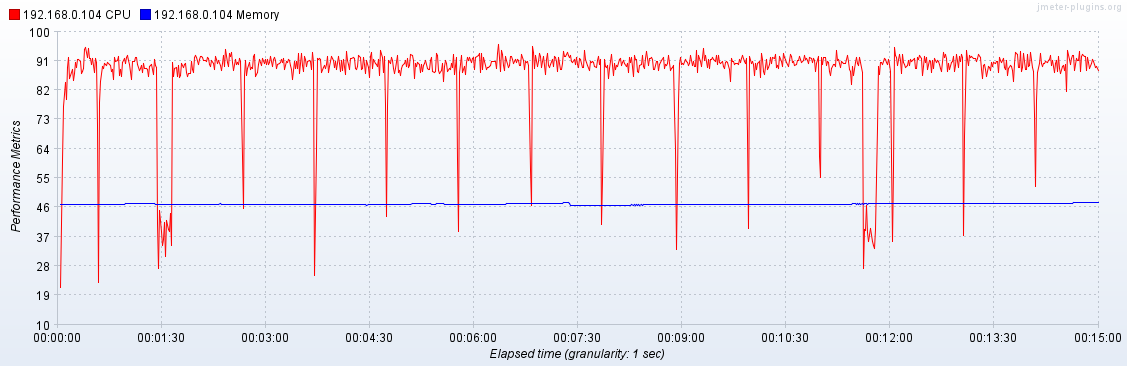
\includegraphics[width=1.0\textwidth]{gfx/perfmon-last-opa.png}
  \caption{Perfmon von Lasttest von Ressource Server mit OPA}
  \label{fig:chapter04:perfmon-last-opa}
\end{figure}

In \autoref{fig:chapter04:perfmon-last-opa} ist die CPU-Auslastung sowie RAM-Belegung während dem Lasttest des Ressource Servers mit entkoppelter Zugriffskontrolle zu sehen. Hier ist zu sehen, dass die CPU-Auslastung deutlich höher ausfällt. Die Zeitachse auf beiden Abbildungen haben jeweils die gleiche Skalierung. Die CPU-Auslastung beträgt hierbei größtenteils ca. 91\%. Dies ist damit zu erklären, dass Open Policy Agent die JSON Web Token, die durch eine HTTP-Verbindung zwischen Server und Open Policy Agent erhalten werden, dekodieren und parsen muss, um eine Zugriffsentscheidung zu treffen. Dieser Vorgang ist anscheinend ressourcenintensiv. Die regelmäßigen Einbrüche der CPU-Auslastung auf unter 50\% sind schwer zu erklären. Die RAM-Belegung entspricht derselben wie in \autoref{fig:chapter04:perfmon-last-noOPA}. Sie bleibt konstant, Memory Leaks und dergleichen treten nicht auf.\smallskip

In beiden Servern wurden alle Anfragen erfolgreich bearbeitet und es kamen keine Fehlermeldungen wie Unerreichbarkeit des Servers vor. Eine erfolgreiche Bearbeitung entspricht hierbei, dass die Server den Token validiert haben und entsprechend erkannt wurde, dass der Nutzer autorisiert ist, eine Antwort von dem Server zu erhalten. Dies entspricht in diesem Fall dem HTTP-Code 200 (OK). 

\section{Skalierbarkeitstest}
In diesem Test wurde eine ansteigende Last auf bis zu 100 Threads auf die jeweiligen Server erzeugt. 

\begin{figure}[H]
  \centering
  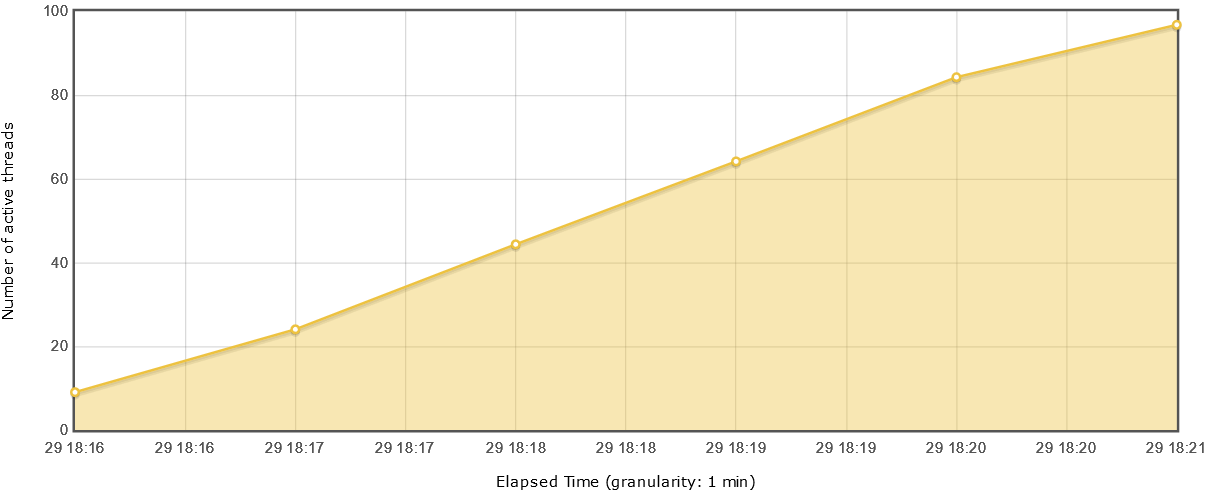
\includegraphics[width=1.0\textwidth]{gfx/flotActiveThreadsOverTime.png}
  \caption{Aktive Threads über Zeitraum des Tests}
  \label{fig:chapter04:flotActiveThreadsOverTime}
\end{figure}

In \autoref{fig:chapter04:flotActiveThreadsOverTime} ist die Anzahl der aktiven Threads über den Zeitraum des Tests dargestellt. Es werden bis zu 100 Threads gestartet und die Anzahl der Threads nimmt kontinuierlich zu. Es wird also eine zunehmende Last auf den Server erzeugt. 

\begin{figure}[H]
  \centering
  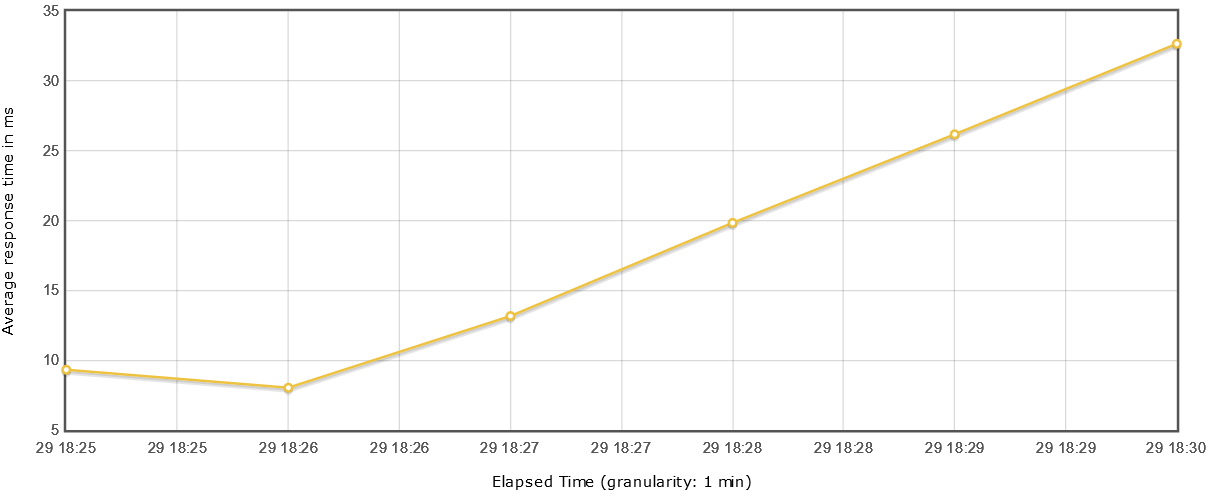
\includegraphics[width=1.0\textwidth]{gfx/flotResponseTimesOverTime-skalierung-noOPA.png}
  \caption{Response Time Graph von Skalierbarkeitstest von Ressource Server ohne OPA}
  \label{fig:chapter04:flotResponseTimesOverTime-skalierung-noOPA}
\end{figure}

In \autoref{fig:chapter04:flotResponseTimesOverTime-skalierung-noOPA} ist ersichtlich, dass bei dem Ressource Server mit interner Zugriffskontrolle die Response Times ab einen gewissen Zeitpunkt kontinuierlich zunehmen. Während sie anfangs lediglich ca. 10 Millisekunden betragen, steigen sie auf bis zu 35 Millisekunden an. Das ist ein relativer Anstieg von 350\% und ein absoluter Anstieg von 25 Millisekunden. 

\begin{figure}[H]
  \centering
  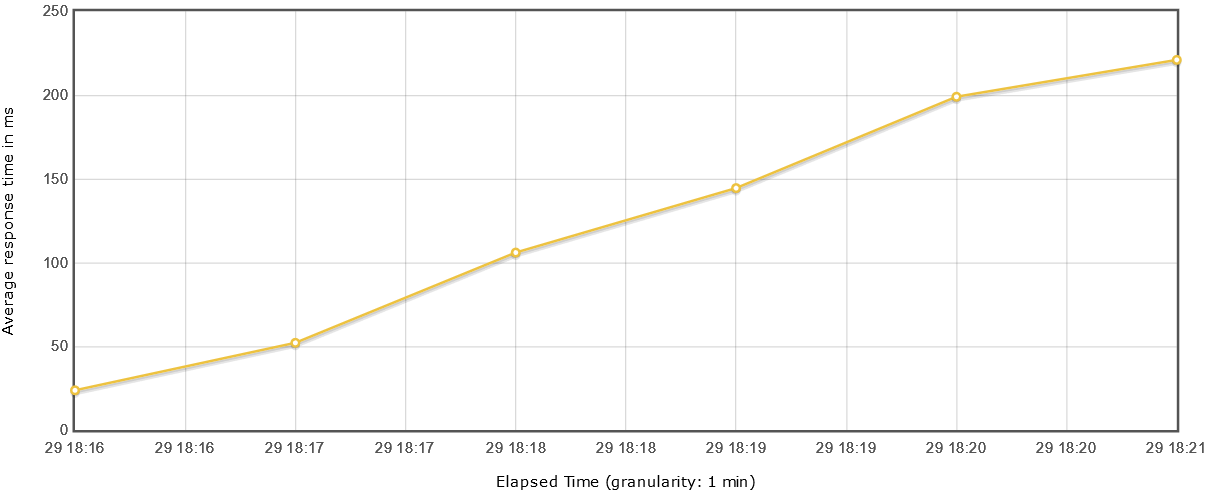
\includegraphics[width=1.0\textwidth]{gfx/flotResponseTimesOverTime-skalierung-opa.png}
  \caption{Response Time Graph von Skalierbarkeitstest von Ressource Server mit OPA}
  \label{fig:chapter04:flotResponseTimesOverTime-skalierung-OPA}
\end{figure}

In \autoref{fig:chapter04:flotResponseTimesOverTime-skalierung-OPA} sind die Response Times für den Ressource Server mit entkoppelter Zugriffskontrolle zu sehen. Hier ist eine ähnliche Situation vorzufinden, nämlich die Response Times steigen kontinuierlich mit steigender Last. Allerdings steigen sie hier von ca. 25 Millisekunden auf bis zu ca. 250 Millisekunden. Das ist ein Anstieg um den Faktor 10 beziehungsweise 1000\% und ein absoluter Anstieg um 225 Millisekunden. Es ist offensichtlich, dass der Server mit entkoppelter Zugriffskontrolle deutlich schlechter skaliert. 

\begin{figure}[H]
  \centering
  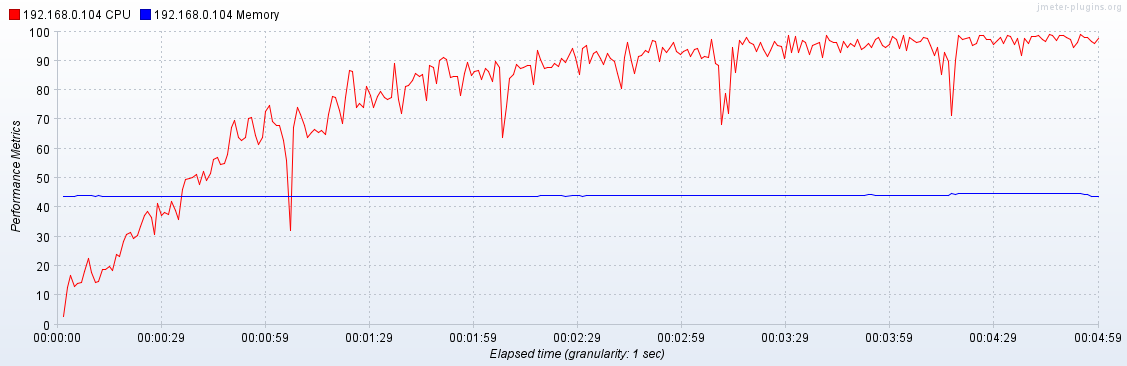
\includegraphics[width=1.0\textwidth]{gfx/perfmon-skalierung-noOPA.png}
  \caption{Perfmon von Skalierbarkeitstest von Ressource Server ohne OPA}
  \label{fig:chapter04:perfmon-skalierung-noOPA}
\end{figure}

In \autoref{fig:chapter04:perfmon-skalierung-noOPA} ist die CPU-Auslastung (rote Linie) im Laufe des Tests bei dem Server ohne Open Policy Agent dargestellt. Es ist ein langsamer Anstieg der CPU-Auslastung festzustellen, die sich auf etwa 95\% einpendelt. 

\begin{figure}[H]
  \centering
  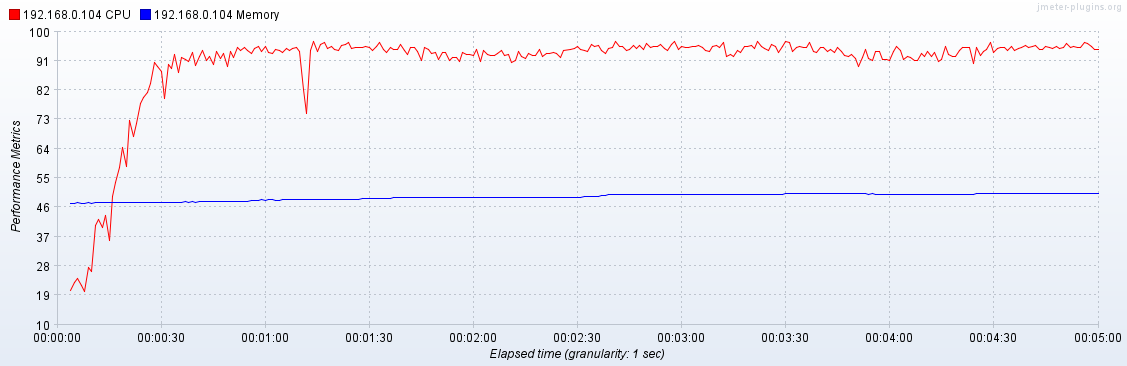
\includegraphics[width=1.0\textwidth]{gfx/perfmon-skalierung-opa.png}
  \caption{Perfmon von Skalierbarkeitstest von Ressource Server mit OPA}
  \label{fig:chapter04:perfmon-skalierung-opa}
\end{figure}

In \autoref{fig:chapter04:perfmon-skalierung-opa} ist die CPU-Auslastung bei dem Server mit Open Policy Agent zu sehen. Hier ist zu sehen, dass die CPU-Auslastung deutlich schneller und steiler ansteigt. Auch daraus kann auf eine schlechtere Skalierung geschlossen werden. 
Die RAM-Belegung bleibt in beiden Systemen jedoch konstant. Dies ist nicht verwunderlich, da Systeme mit JSON Web Token als statuslos gelten, das heißt, dass der Server keine Informationen des Clients speichern muss, da alle Informationen in dem JSON Web Token vorhanden sind. 
Ein weiterer äußerst erwähnenswerter Punkt ist der, dass während des Skalierbarkeitstests, zeitweise Open Policy Agent unerreichbar war. 

\begin{figure}[H]
  \centering
  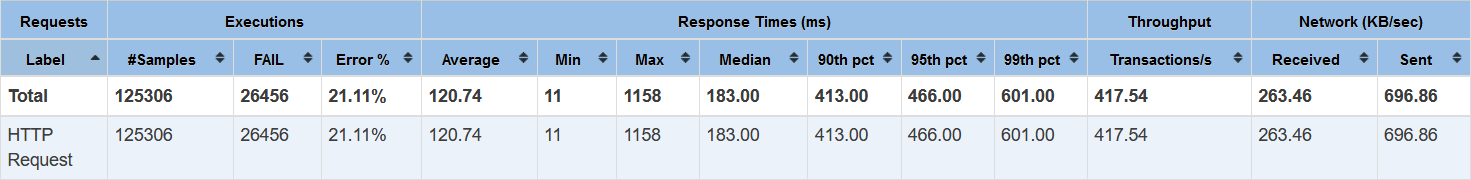
\includegraphics[width=1.0\textwidth]{gfx/statistik-skalierung-opa.png}
  \caption{Statistiken von Skalierbarkeitstest von Ressource Server mit OPA}
  \label{fig:chapter04:statistik-skalierung-opa}
\end{figure}

In dem Server, der die Zugriffskontrolle mit Open Policy Agent entkoppelt hat, wurden 21,11\% aller Anfragen nicht erfolgreich beantwortet, stattdessen wurden sie mit dem HTTP-Code 500 beantwortet. Der Fehler-Code 500 steht für Internal Server Error \citep{mdnwebdocs:2021}. Die Ursache davon ist, dass der Ressource Server, also die Spring-Boot-Applikation, nicht Open Policy Agent erreichen konnte. 

\begin{lstlisting}[frame=tb,caption={Fehlermeldung Spring-Boot},label=lst:FehlermeldungSpring-Boot]
  org.springframework.web.client.ResourceAccessException: I/O error on POST request for "HTTP://localhost:8181/v1/data/HTTP/authz/allow": Address already in use: connect; nested exception is java.net.BindException: Address already in use: connect
\end{lstlisting}
\bigskip

Die Meldung, die die Spring-Boot Applikation, ausgibt ist in \autoref{lst:FehlermeldungSpring-Boot} zu sehen. Der Ressource Server sendet jeweils bei jeder einkommenden Anfrage von Clients eine HTTP-POST Anfrage an Open Policy Agent, um eine Zugriffsentscheidung für diese Anfrage des Clients zu erhalten. Dies war in 21.11\% aller Anfragen nicht möglich, weil Open Policy Agent blockiert. Da dieses Verhalten bei dem Lasttest nicht aufgetreten ist und der Lasttest mit lediglich zehn Threads eine weitaus geringere Belastung generiert, ist davon auszugehen, dass ab einer gewissen Belastung Open Policy Agent sperrt.\smallskip

Open Policy Agent selbst nutzt als Webserver kein Apache Tomcat, sondern einen eigens in Go programmierten Webserver \citep{opagithub:2021}. Etwaige Performanceeinstellungen lassen sich nicht vornehmen, ohne den Source-Code zu modifizieren und Open Policy Agent neu zu kompilieren und ein Docker-Container daraus wieder zu erstellen. 

\section{Stresstest}
Bei dem Stresstest wurde eine abnormal hohe Belastung auf beide Server erzeugt, um die Grenzen des Systems auszuloten. Hier wurden 1000 Threads über einen Zeitraum von 15 Minuten gestartet. 

\begin{figure}[H]
  \centering
  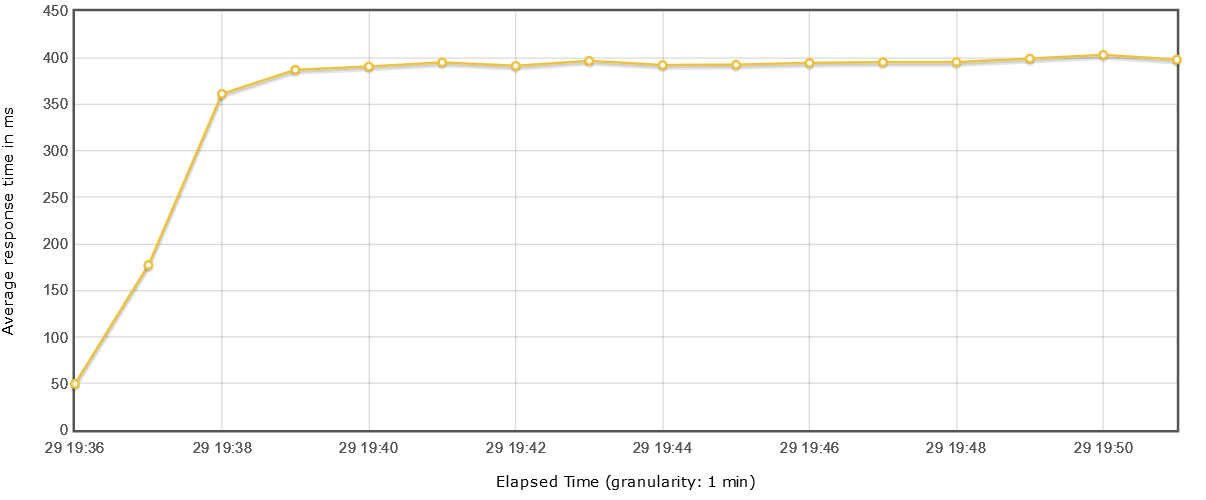
\includegraphics[width=1.0\textwidth]{gfx/flotResponseTimesOverTime-stress-noOPA.png}
  \caption{Response Time Graph von Stresstest von Ressource Server ohne OPA}
  \label{fig:chapter04:flotResponseTimesOverTime-stress-noOPA}
\end{figure}

In \autoref{fig:chapter04:flotResponseTimesOverTime-stress-noOPA} sind die Response Times für den Server ohne OPA über den Zeitraum des gesamten Stresstests dargestellt. Die Response Times stiegen kontinuierlich an, bis sie sich auf etwa durchschnittlich 400 Millisekunden einpendeln. 

\begin{figure}[H]
  \centering
  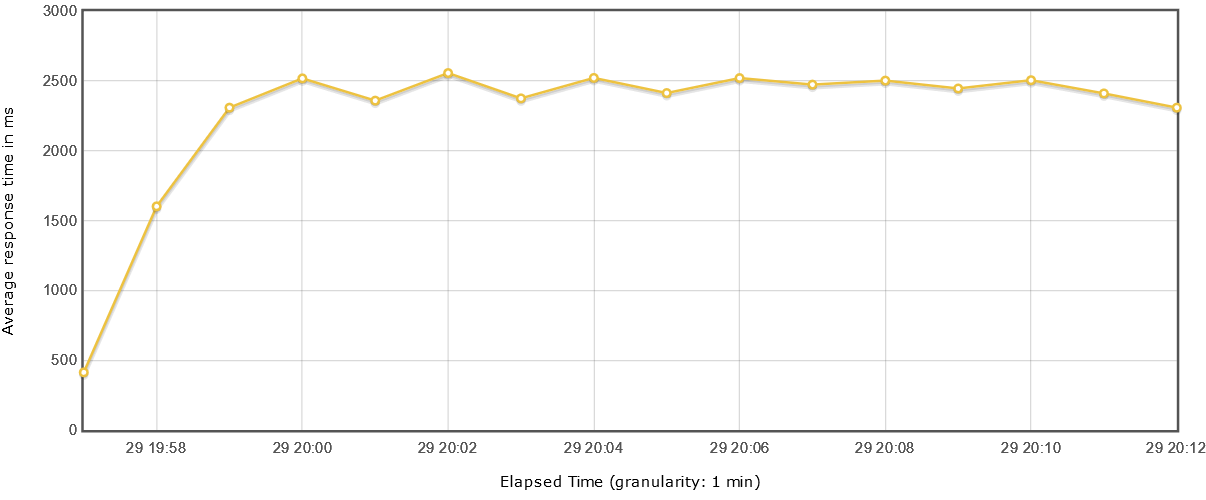
\includegraphics[width=1.0\textwidth]{gfx/flotResponseTimesOverTime-stress-opa.png}
  \caption{Response Time Graph von Stresstest von Ressource Server mit OPA}
  \label{fig:chapter04:flotResponseTimesOverTime-stress-opa}
\end{figure}

In \autoref{fig:chapter04:flotResponseTimesOverTime-stress-opa} sind die Response Times für den Server mit entkoppelter Zugriffskontrolle mit Open Policy Agent zu sehen. Das Verhalten ist insgesamt sehr ähnlich, das heißt die Response Times steigen bis zu einem gewissen Zeitpunkt und bleiben dann konstant. Hier pendeln sich die Response Times allerdings auf 2500 Millisekunden ein. Das bedeutet im Vergleich zu dem Server ohne entkoppelter Zugriffskontrolle, sind diese Response Times ca. 6,25-mal höher. 

\begin{figure}[H]
  \centering
  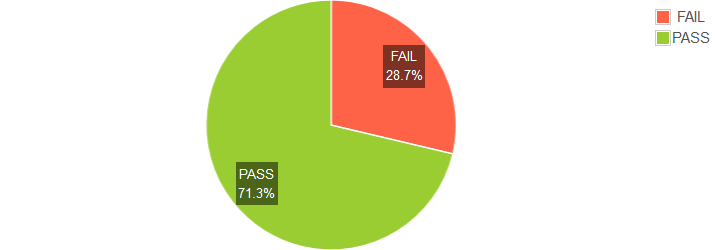
\includegraphics[width=1.0\textwidth]{gfx/requests-summary-stress-opa.png}
  \caption{Request Summary von Stresstest von Ressource Server mit OPA}
  \label{fig:chapter04:requests-summary-stress-opa}
\end{figure}

Allerdings wurden auch bei dem Stresstest ähnlich wie bei dem Skalierbarkeitstest eine hohe Anzahl von Anfragen bei dem Server mit entkoppelter Zugriffskontrolle nicht erfolgreich beantwortet. Dies ist in \autoref{fig:chapter04:requests-summary-stress-opa} erkenntlich. 28,7\% aller Anfragen wurden nicht erfolgreich beantwortet. Auch hier war Open Policy Agent schlichtweg nicht erreichbar für den Server, sodass der Server dem Client mit dem HTTP-Code 500 antwortete.
Aufgrund der hohen Response Times und den nicht erfolgreich beantworteten Anfragen, ist der Application Performance Index bei dem Server mit Open Policy Agent deutlich schlechter ausgefallen. 

\begin{figure}[H]
  \centering
  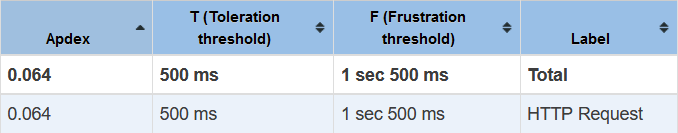
\includegraphics[width=1.0\textwidth]{gfx/APDEX (Application Performance Index)-stress-opa.png}
  \caption{APDEX (Application Performance Index) von Stresstest von Ressource Server mit OPA}
  \label{fig:chapter04:APDEX (ApplicationPerformanceIndex)-stress-opa}
\end{figure}

Der Application Performance Index für das System mit Open Policy Agent ist in \autoref{fig:chapter04:APDEX (ApplicationPerformanceIndex)-stress-opa} zu sehen. Lediglich weniger als 6.4\% aller Anfragen wurden bei diesem Server mit einer Response Time von weniger als 500 Millisekunden beantwortet. In anderen Worten: Der Großteil aller Antworten der Anfragen dauern aus Nutzersicht zu lange, sodass diese Nutzer frustriert sind.

\begin{figure}[H]
  \centering
  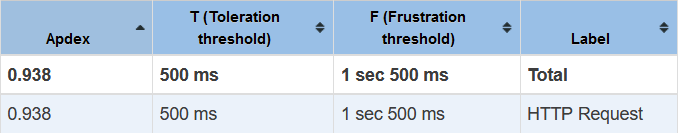
\includegraphics[width=1.0\textwidth]{gfx/APDEX (Application Performance Index)-stress-noOPA.png}
  \caption{APDEX (Application Performance Index) von Stresstest von Ressource Server ohne OPA}
  \label{fig:chapter04:APDEX (ApplicationPerformanceIndex)-stress-noOPA}
\end{figure}

Bei dem Server ohne entkoppelter Zugriffskontrolle hingegen, fällt der Score des Application Performance Index mit 0.938 wesentlich besser aus, siehe \autoref{fig:chapter04:APDEX (ApplicationPerformanceIndex)-stress-noOPA}. Fast alle Anfragen konnten hier innerhalb von 500 Millisekunden erfolgreich beantwortet werden. 

\section{Ressource Server und OPA in Kubernetes Cluster}

In diesem Kapitel wird gesondert betrachtet, inwiefern sich ein Deployment von Ressource Server und OPA in einem Kubernetes Cluster auf die Performancewerte auswirkt. Hierbei befindet sich Ressource Server und OPA in demselben Pod. OPA wird also als Sidecar verwendet. 

\begin{figure}[H]
  \centering
  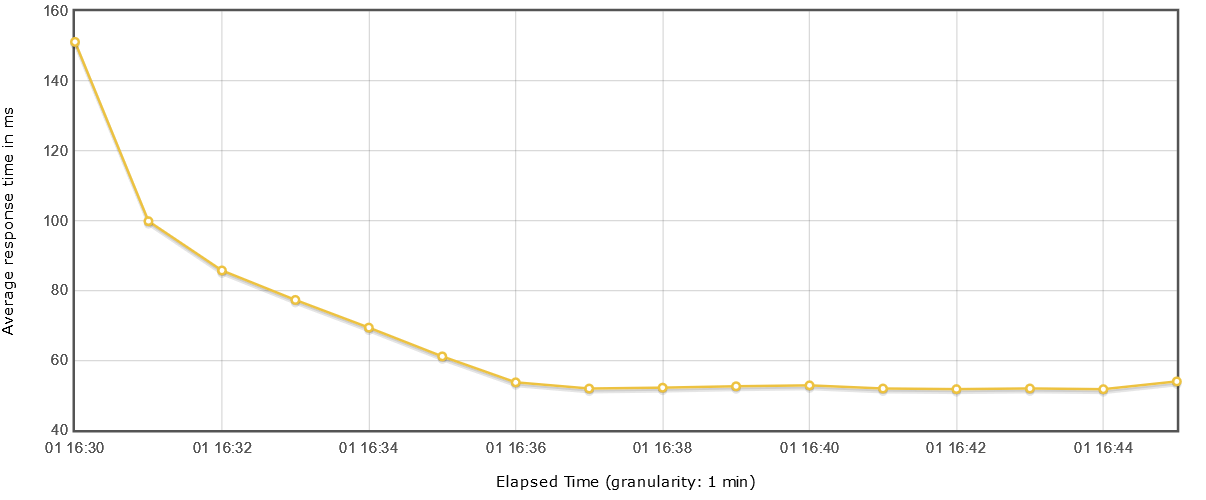
\includegraphics[width=1.0\textwidth]{gfx/flotResponseTimesOverTime-opa-last-k8s.png}
  \caption{Response Time Graph von Lasttest von Ressource Server mit OPA in einem Kubernetes Cluster}
  \label{fig:chapter04:flotResponseTimesOverTime-opa-last-k8s}
\end{figure}

In \autoref{fig:chapter04:flotResponseTimesOverTime-opa-last-k8s} ist der Response Time von dem Lasttest abgebildet. Es ist zu sehen, dass hier die Response Times deutlich höher ausfallen im Vergleich zu \autoref{fig:chapter04:statistik-last-opa}. Auffallend ist außerdem, dass die Response Times kontinuierlich abnehmen, bis sie sich auf ca. 55 Millisekunden einpendeln. 

\begin{figure}[H]
  \centering
  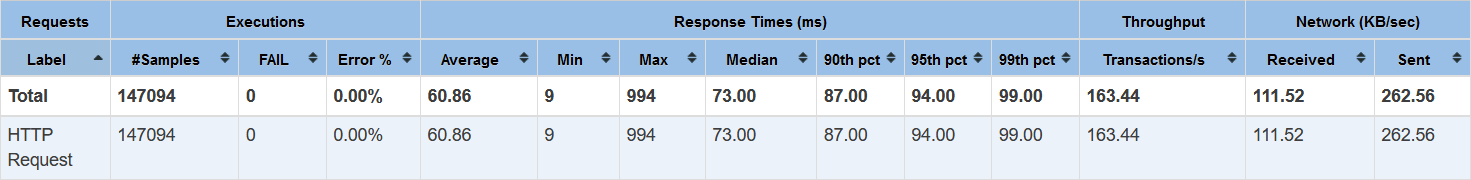
\includegraphics[width=1.0\textwidth]{gfx/statistik-last-opa-k8s.png}
  \caption{Statistiken von Lasttest von Ressource Server mit OPA in Kubernetes Cluster}
  \label{fig:chapter04:statistik-last-opa-k8s}
\end{figure}

In \autoref{fig:chapter04:statistik-last-opa-k8s} sind die Gesamtstatistiken des Lasttests zu sehen. Die durchschnittliche beträgt hier ca. 60 Millisekunden während sie bei dem System ohne Kubernetes lediglich durchschnittlich 27 Millisekunden betragen, siehe \autoref{fig:chapter04:statistik-last-opa}.\smallskip

Bei dem Skalierbarkeitstest fielen die Response Times ebenfalls weitaus höher aus, diese werden hier allerdings nicht weiter diskutiert. Die Statistiken und Graphen können dem \autoref{Appendix} entnommen werden. Was allerdings erwähnenswert ist, ist das während des Skalierbarkeitstest OPA immer verfügbar war, was bei demselben Test in dem System ohne Kubernetes nicht der Fall gewesen ist. Dies ist durch die Nutzung der Replica zu begründen, denn hier wurde ein LoadBalancer verwendet der gleichmäßig die Anfragen auf die zwei Instanzen des Pods verteilt. 

\begin{figure}[H]
  \centering
  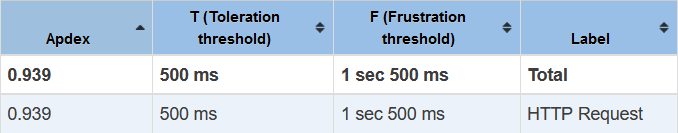
\includegraphics[width=1.0\textwidth]{gfx/APDEX (Application Performance Index)-skalierung-OPA-k8s.png}
  \caption{APDEX (Application Performance Index) von Skalierbarkeitstest von Ressource Server mit OPA und Kubernetes}
  \label{fig:chapter04:Application Performance Index)-skalierung-OPA-k8s}
\end{figure}

Dadurch hat sich auch der Application Performance Index verbessert, wie es in \autoref{fig:chapter04:Application Performance Index)-skalierung-OPA-k8s} zu sehen ist. Dieser beträgt 0.939. 

\begin{figure}[H]
  \centering
  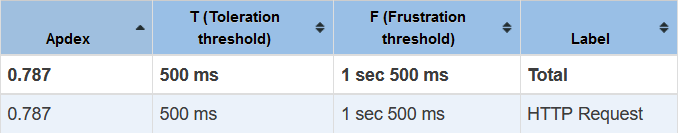
\includegraphics[width=1.0\textwidth]{gfx/APDEX (Application Performance Index)-skalierung-OPA.png}
  \caption{APDEX (Application Performance Index) von Skalierbarkeitstest von Ressource Server mit OPA ohne Kubernetes}
  \label{fig:chapter04:APDEX (Application Performance Index)-skalierung-OPA}
\end{figure}

In \autoref{fig:chapter04:APDEX (Application Performance Index)-skalierung-OPA} ist der Application Performance Index des Skalierbarkeitstest des Systems mit OPA aber ohne Kubernetes zu sehen. Hier fiel der Index mit 0.787 deutlich schlechter aus aufgrund der Nichtverfügbarkeit von OPA.\smallskip

Der Stresstest fiel ebenfalls schlechter aus in allen Belangen, dieser wird hier allerdings nicht näher erläutert. Die entsprechenden Messergebnisse können allerdings dem \autoref{Appendix} entnommen werden. 

\section{Fazit}
Es konnte gezeigt werden, dass eine entkoppelte Zugriffskontrolle mittels Open Policy Agent in einem OAuth2 System einen signifikanten negativen Einfluss auf die Performance hat. Bei leichter Last mit lediglich zehn gleichzeitigen Threads, fallen die Response Time durchschnittlich um ein dreifaches höher aus als bei dem Ressource Server, der die Zugriffskontrolle in der Spring-Boot Applikation implementiert hat.\smallskip

Monolithen sind zwar grundsätzlich schneller als Microservice Architekturen durch die hinzukommende HTTP-Kommunikation zwischen den Microservices, aber ein derartig großer Performanceunterschied wurde nicht erwartet unter dem Hintergrund, dass bei dem Ressource Server mit entkoppelter Zugriffskontrolle, der Server und Open Policy Agent auf demselben Host laufen. Zu erwähnen ist hierbei allerdings, dass wenn jeweils auf die Response Time eine entfernungsabhängige Latenz zwischen Client und Server hinzugerechnet wird, der prozentuale Unterschied in der Performance zwischen Server mit interner vs. externer Zugriffskontrolle, geringer ist. Zusätzlich muss beachtet werden, dass die hier programmierte http-GET-Schnittstelle in den jeweiligen Servern äußerst rudimentär ist. Das bedeutet, es wird keine lange Rechenzeit benötigt, die die Response Time maßgeblich beeinflusst. Auch dies kann in anderen Szenarien anders sein und den relativen Unterschied in der Performance zwischen beiden Servern verringern.\smallskip

Neben der Response Time fiel zudem die äußerst hohe CPU-Auslastung im System mit entkoppelter Zugriffskontrolle auf. Bei dem Lastttest ist diese doppelt so hoch im Vergleich zu dem Server ohne Open Policy Agent. Selbst bei nur zehn gleichzeitig Threads bewegt sich das System mit Open Policy Agent bei annähernd 100-prozentiger CPU-Auslastung beinahe am Anschlag.\smallskip

Zudem sperrt der Server von Open Policy Agent ab einer bestimmten Belastung, sodass der Ressource Server viele Client-Anfragen mit einer HTTP-Fehlermeldung 500 beantworten musste. Es scheint, dass mehrere Instanzen von Open Policy Agent für einen einzigen Ressource Server erstellt werden müssen, damit das Gesamtsystem unter starker Last regulär funktioniert. Da allerdings schon bei zehn Threads, das System mit Open Policy Agent am Anschlag arbeitet, scheint es nicht sinnvoll, mehrere Instanzen von Open Policy Agent auf der gleichen Host-Maschine zu starten. Wenn allerdings mehrere Open Policy Agent Instanzen auf mehreren Hosts laufen, würde die Latenz zwischen Ressource Server und Open Policy Agent zunehmen, da diese ja wiederrum nicht mehr auf dem gleichen Host laufen. Es scheint also, dass bei der Nutzung von Open Policy Agent unweigerlich ein Kompromiss eingegangen werden muss.\smallskip

Eine Verbesserung der Performance durch ein Deployment von Ressource Server und OPA in einem Kubernetes Cluster konnte nicht erreicht werden. Zwar konnte die Verfügbarkeit zumindest in dem Skalierbarkeitstests verbessert werden, allerdings fielen die Response Times in allen Fällen deutlich höher aus als in dem System, das kein Kubernetes verwendet. Dies ist auf den zusätzlichen Kommunikationsaufwand zurückzuführen, denn die Serices in einem Kubernetes Cluster sind nicht direkt erreichbar, sondern der LoadBalancer leitet Anfragen entsprechend an die Ports der Pods weiter. Dadurch ist zwar eine horizontale Skalierung möglich, allerdings ist dies logischerweise in einem Cluster, dass lediglich ein Node besitzt wenig effektiv. 
